\documentclass[11pt,paper,footinclude=true,headinclude=true,oneside]{scrbook} % KOMA-Script book
\usepackage[T1]{fontenc}                
\usepackage{lipsum}
\usepackage[linedheaders,parts,pdfspacing]{classicthesis} % ,manychapters
%\usepackage[osf]{libertine}
\usepackage{amsthm}
\usepackage{graphicx,listings,accents,tikz,multicol}
\usepackage{subcaption,tcolorbox}
\tcbuselibrary{theorems}
\usetikzlibrary{decorations.pathreplacing}

\newtcbtheorem{mytheorem}{\emph{Theorem:}}{colback = blue!10, colframe = blue!50!black, fonttitle = \bfseries}{th}
\newtcbtheorem{mydefinition}{\emph{Definition:}}{colback=red!5!white,colframe=red!45!white, title = Myboxy, fonttitle = \bfseries}{defi}
\newtcbtheorem{myobservation}{\emph{Observation:}}{colback = tachameleon, colframe = blue!40!white, fonttitle = \bfseries}{rem}
\usepackage{setspace}
\usepackage[rgb]{xcolor}
\usepackage{verbatim}
\usepackage{amsgen,amsmath,amstext,amsbsy,amsopn,amssymb,tkz-linknodes,fancyhdr}
\usetikzlibrary{arrows, calc, babel, shapes}
\usepackage[colorlinks=true, urlcolor=blue,  linkcolor=blue, citecolor=blue]{hyperref}
\usepackage[colorinlistoftodos]{todonotes}
\usepackage[fulladjust]{marginnote}
\usepackage{rotating}
\usepackage{listings}
\usepackage[utf8]{inputenc}
\usepackage{amsmath,amsthm,amsfonts,amssymb,amscd,babel,float}
\usepackage{paracol,tikz}
\usepackage{tkz-fct}
\usepackage{fancyhdr}
\usepackage[top=2cm, bottom=4.5cm, left=2.5cm, right=2.5cm]{geometry}
\usepackage{xstring}
\pagestyle{fancyplain}

\newcommand*{\titleGP}{\begingroup % Create the command for including the title page in the document
\centering % Center all text
\vspace*{\baselineskip} % White space at the top of the page


\rule{\textwidth}{1.6pt}\vspace*{-\baselineskip}\vspace*{2pt} % Thick horizontal line
\rule{\textwidth}{0.4pt}\\[\baselineskip] % Thin horizontal line

{\LARGE Growth theory}\\[0.2\baselineskip] % Title
{ \Large  Jakub Pawelczak }\\[0.2\baselineskip] % Title
\rule{\textwidth}{0.4pt}\vspace*{-\baselineskip}\vspace{3.2pt} % Thin horizontal line
\rule{\textwidth}{1.6pt}\\[\baselineskip] % Thick horizontal line

\scshape % Small caps
Lecture notes\\[\baselineskip] % Tagline(s) or further description

\vspace{2 cm}

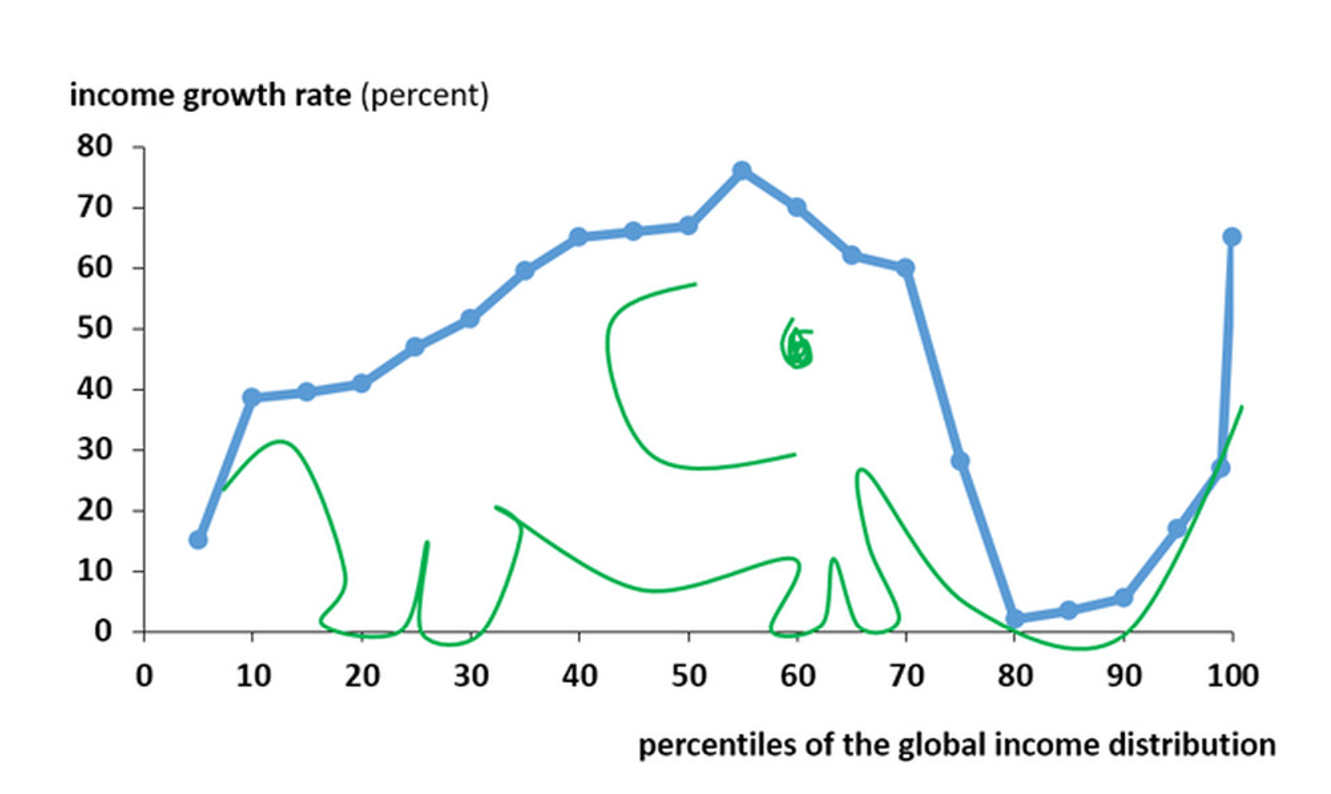
\includegraphics[scale=0.7]{title1.png} \\[0.5\baselineskip]


\vspace*{2\baselineskip} % Whitespace between location/year and editors

\\


\vfill % Whitespace between editor names and publisher logo

\includegraphics[scale=0.7]{sgh.jpg} \\[0.3\baselineskip] 
Warsaw \today \par % Location and year\\
{ Typed by Kuba Pawelczak \par} % Editor list

\endgroup}



\begin{document}
\titleGP
%\pagestyle{empty}


	\pagestyle{scrheadings}
%	\manualmark
%	\markboth{\spacedlowsmallcaps{\contentsname}}{\spacedlowsmallcaps{\contentsname}}
	
	\tableofcontents 

%	\automark[section]{chapter}
%	\renewcommand{\chaptermark}[1]{\markboth{\spacedlowsmallcaps{#1}}{\spacedlowsmallcaps{#1}}}
%	\renewcommand{\sectionmark}[1]{\markright{\thesection\enspace\spacedlowsmallcaps{#1}}}

    % use \cleardoublepage here to avoid problems with pdfbookmark
   
 
   
\newcommand{\ImageWidth}{15cm}
\part{Empirics of Economic Growth}
\chapter{Overview of Growth Theory}
\input{growth1}
\part{Exogenous Growth Models}
\chapter{Solow and Mankiw-Romer-Weil Models}
\input{growth2}
\chapter{Pontryagin Maximum Principle}
\input{growth3}
\chapter{Ramsey Model}
\input{growth4}
\part{Endogenous Growth Models}
\chapter{Endogenous Growth. AK Model}
\input{growth5}
\chapter{Jones-Manuelli Model. Uzawa-Lucas Model. Growth with Externalities }
\input{growth6}
\chapter{Endogenous Technical Change. Romer Model}
\input{growth7}
\chapter{Schumpeterian (Quality Ladder) Growth Model }
\input{growth8}
\chapter{Uzawa Balanced Growth Theorem}
\input{growth9}
\chapter{Scale effects.Jones critique}
\input{growth10}
\chapter{Convergence. Technology Diffusion}
\input{growth11}
\begin{thebibliography}{9}
TBD
\end{thebibliography}
\end{document}